% Chapter 5

\chapter{Derivation of Schematics from Hardware Requirements} % Main chapter title

\label{Chapter5} % Change X to a consecutive number; for referencing this chapter elsewhere, use \ref{ChapterX}

This chapter provides a detail description and insight into the derivation of the schematics based on the hardware requirements. This includes describing how each schematic was created, and its purpose, as well as how each component was selected.

%----------------------------------------------------------------------------------------
%	SECTION 1
%----------------------------------------------------------------------------------------

\section{Designing the Schematics}

	All of the following schematics that will be mentioned in this section were designed using Altium Designer 18. The use of component datasheets and online tutorials aided in the design as well as input from the Academic Supervisor. Most of the schematic and PCB models were either downloaded from the manufacturer's website or from SnapEDA. The following paragraphs will give an overview of the various schematics and why they were designed and for what purpose they have with the MEGA65 phone.

\subsection{FPGA Pins}
\label{chap:FPGA}
	The FPGA pins were designed to be connected to the Nexys FPGA board and are the sole CPU of the device. This part of the device will have the Nexys FPGA board plugged into the top of it.\\
Being the overall connection sheet for the phone, the FPGA pin sheet was labelled as the top sheet. The FPGA would be the main CPU of the board with most components on the phone needing a connection to an FPGA pin. Two 50-Pin headers were placed on the schematic which mimicked the pin connection on the FPGA board. Some of the connections to other components included the I2C connections (data and clock lines), PCM connections, UART connections and the red, green and blue connections for both the VGA connection and LCD screen.\\
The schematic of the component was designed for the project while the footprint was found pre-made. 

\subsection{Power Control Circuitry}
\label{chap:batt}
	The Power Control circuitry was designed to ensure that certain devices could be switched off if required, and also to ensure that adequate power was being supplied to all necessary components on the device. To begin a number of voltage regulators were added to the schematic as well as a flip-flop to be used for the main FPGA power. A I2C I/O Expander was also used in the schematic so that all the voltage regulators could be connected to it.\\

	The circuitry was connected up by first connecting a slide switch between the shutdown and power lines of the voltage regulator. An LED was then connected to the output line to ensure that if the regulator was powered an LED would illuminate, with the output line producing the required power rail needed. This was repeated six times to create the multiple power rails required for all the different components.\\

	There were a few changes made to the power control circuitry after going through and analysing all the schematics. It was found that the voltage regulator would only give out 0.1A of current wheras the modems would need at least 2A of current, 4A at best. The circuitry was updated to include the new part found so that the output current would be adequate for the modems. 

\subsection{Charging Circuitry}

	Parts of the schematic for the charging circuit were already completed by a student in a previous year. The schematic was checked over for errors and against the datasheet of the main component so that everything would work as expected. It was decided early on that the majority of this schematic would be completed by a professional, due to its complexity.

\subsection{Voltage Step-Up}

	The Voltage Step-up was required as a few of the components require 5V. This was completed by using an NCP1402 and connecting VCC MIC to the input voltage line. The rest of the circuitry was completed by following the recommended layout in the datasheet. The use of the NCP1402 was based on a recommendation written in a past student's thesis, with the component being verified for its usability in the phone. 

\subsection{Signal Connections}

	The Signal Connections schematic was designed to contain all the off-sheet connectors from the various components which operated through I2C and Interrupt lines. The separate signals were connected together with resistor pull-ups added to the two I2C lines. The output of these signals were all sent directly to FPGA pins. 

\subsection{I2C I/O Expanders}

	There were a number of I/O Expanders which were added to the device. These were added to add in a number of peripherals which didn't necessarily need to be connected to FPGA pins. There were a number of expanders due to all the pins on a particular expander needing to have the same inout/output source. 
The I/O Expanders were added into the schematics to allow the device to have more connections. The DPAD and buttons were connected to an I/O Expander with the use of resistor pull-ups. A number of other signals which were required to be active while the FPGA was active, were added to another I/O Expander.

\subsection{VGA Connection}
\label{chap:VGA}
	The VGA was connected using a 15-Pin DSUB connector. A resistor ladder was used for the colour connections with the signals going straight out to the FPGA board. Resistor values of 4k, 2k and 510 Ohms were used for the ladder with two 0 Ohm resistors used for the HSYNC and VSYNC lines. The datasheet for the VGA connection was used as a basis for the signal connections. 
 
\subsection{LCD Display}
\label{chap:LCD}
	The LCD Display schematic was connected in a similar way as the VGA connection with resistor pull-ups used for all three colour connections. The purpose of the schematic would be to provide the LCD display for the phone.

\subsection{Touch Screen}
\label{chap:touch}
	The Touch Screen was added to the schematic to give the ability to the user to use their fingers for functionality, as well as the thumbpad and buttons. 
The Touch Screen connection was completed by powering it with VCC Screen and adding in I2C signals and an Interrupt line, going to the Signal Connections sheet.

\subsection{LED Backlight Display}

	The LED Backlit Display was designed using a simplified design already created by another producer. This circuit was designed to provide a backlit display when the phone is on and to dim the screen when the phone is in a call or facing down.

\subsection{Accelerometer}
\label{chap:a}
	The accelerometer was designed mainly through reading the recommended application layout in the datasheet of the component. Off-sheet connectors were used for the I2C signals and the Interrupt lines, as well as the three ADC lines which were used for the volume thumbwheel. The power for the component was connected to the VCC MIC power rail.

\subsection{Real-Time Clock}
\label{chap:RTC}
	The schematic connections for the RTC were made by following the typical application layout given in the manufacturer's datasheet.

\subsection{Proximity Sensor}
\label{chap:prox}
	The schematic and PCB models for the Proximity Sensor were accessed from the internet with all the connections followed from the manufacturer's datasheet. 

\subsection{4G Modems}
\label{chap:modem}
	4G modems were added to the device to enable 4G internet connection. Two 4G modems were added to the schematics so that the user would have the ability to be connected to two different networks at once.
The schematic for the 4G modem was downloaded off the internet with many of the connections also being read off the manufacturer's datasheet. 

\subsection{WiFi Module}

	The WiFi module was added into the schematics to enable the phone to have WiFi capability. This module was connected through the GPIO bits and an I2C connection.

\subsection{NOR Flash}

	The NOR Flash schematic was designed to have primary use within the One-Time Pad encryption. The component would have no other function on the phone. 

\subsection{Barometer}

	The schematic connections for the Barometer were completed by following the recommended layout given on the manufacturer's datasheet. 

\subsection{LoRa Radio}

	The two LoRa Radios were connected up using the recommended application layout given by the manufacturer's datasheet. The UART connections were made directly to the FPGA pins.

\subsection{MEMs Microphones}
\label{chap:mics}
	The two MEMs Microphones were connected by following the datasheet's guidelines. The individual data lines were sent straight to the FPGA, while the two clock lines were tied together and sent to the FPGA board. 

\subsection{Headphone Audio Filter} 
\label{chap:audio2}
	The Headphone Audio Filter was created by following the design of a Sallen-Key Lowpass Filter, with two being designed. A chip containing two amplifiers was used for the design with the output of both chips being the left and right headphone audio respectively. 

\subsection{Audio Power Amplifier}
\label{chap:audio}
	The schematic for the Audio Power Amplifier was completed using a number of recommended layouts found in the component's recommend layout and recommended schematics found across the internet. This schematic was designed to produce the audio for the phone. 

\subsection{Digital Compass}

	The Digital Compass was added to give the device the use of a compass which would be used for both gyroscopic effect and the location of the device.
Like many of the other components the signal connections on the schematic were wired using the recommended application layout. 

\subsection{Bluetooth Module}

	The Bluetooth module was added into the schematic to ensure that the device would be compatible with Bluetooth. This would allow the user to connect to a third-party peripheral device.
The circuitry for the Bluetooth module was created by following the recommend layout on the component's datasheet. The UART and PCM connections were made directly to FPGA pins. 

\subsection{SIM Card Connection}
\label{chap:SIM}
	
%----------------------------------------------------------------------------------------
%	SECTION 2
%----------------------------------------------------------------------------------------

\section{Component Selection} 
	
	This section describes the major components selected for the phone. This also includes other components which were compared and tested so that the optimal solution would be found. 

%----------------------------------------------------------------------------------------
%	SUBSECTION 1
%----------------------------------------------------------------------------------------

\subsection{Resistor and Capacitor Selection}

It was decided early on that (where possible) that all resistors and capacitors would be 0805 sized. This would maintain the aesthetic look of the PCB, as well as reduce hassle with the order and delivery of components. 

%----------------------------------------------------------------------------------------
%	SUBSECTION 2
%----------------------------------------------------------------------------------------

\subsection{Power Supply Option}

	There were a number of different options that could have been chosen for the power supply. The proposed idea for the supply circuit was to have multiple power supplies for all the major components of the device. It was found through analysing the circuit after completing the main portion of the schematics that the current output would have to be at least 4A to account for the modems. However, in most circumstances the modems would probably still work fine with 2A. There were some issues trying to find a power supply option that both could output at least 2A of current and could be SMD soldered in a regular fashion. 

\subsubsection{TPS6302x High Efficiency Single Inductor Buck-Boost Converter}

It was proposed early on that multiple Texas Instruments TPS6302x High Efficiency Single Inductor Buck-Boost Converters with 4-A Switches would be used as the power supply. One was designed for both of the cellular radios, one to power WiFi and Bluetooth, one for the FPGA board, one connected to the battery source and two for the modems. 
This option was given priority over the other power supplys due to it having a 2A enable line, and after analysing the other power supply options was used as the power supply option. 


\subsubsection{CDMA Cellular/PCS System Power Supplies}

This power supply was considered however the power supplies are designed specifically for CDMA cellular/PCD handsets. For this reason, these power supplies were deemed to be not sufficient for the purposes of the phone. 

\subsubsection{TPS6128xA Low-, Wide- Voltage Battery Front-End DC/DC Converter Single-Cell Li-Ion, Ni-Rich, Si-Anode Applications}

The LP2951 voltage regulator was chosen as the regulator due to it having a low quiescent current and a low dropout voltage. The regulator also is ideally suited to work in battery-powered systems. 

\subsubsection{LP2951-N Adjustable Micropower Voltage Regulator}

The LP2951 voltage regulator was chosen intially as the regulator due to it having a low quiescent current and a low dropout voltage. It was also chosen as it was readily available and easy to obtain. The regulator also is ideally suited to work in battery-powered systems. Later on in the project it was found that the regulator didn't provide enough current to supply to the Wi-Fi module and the modems, because of this an alternative was found which would supply the correct current.


\subsubsection{TPS63805 High Current, High Efficiency Single Inductor Buck-Boost Converter}

After discovering that the LP2951 voltage regulator wouldn't be sufficient for the project the TPS63805 was chosen instead as it would provide a high enough current to be able to work with both the two modems and the Wi-Fi module. However, this module was in DSBGA form and was unsuitable for the device due to its soldering requirements. 


%----------------------------------------------------------------------------------------
%	SUBSECTION 3
%----------------------------------------------------------------------------------------

\subsection{4G Modem}
\subsubsection{ QUECTEL EC25-AU}

	This module was chosen based upon research completed by other students in previous reports. This modem was also being used in the bench-top prototype, and already familiar with most of the software developed. 
%----------------------------------------------------------------------------------------
%	SUBSECTION 4
%----------------------------------------------------------------------------------------

\subsection{Wi-Fi Module}
\subsubsection{}
		This module was also chosen based upon research completed by other students in previous reports. Again, this module was already being used in the bench-top prototype and familiar with the software being developed for it. 

%	SUBSECTION 5
%----------------------------------------------------------------------------------------

\subsection{Bluetooth Module}
\subsubsection{RN52 Module}
	This module was chosen based of its use for simple, mobile devices and its cost. There weren't many other alternatives that provided the same features. 

%----------------------------------------------------------------------------------------
%	SUBSECTION 6
%----------------------------------------------------------------------------------------

\subsection{LoRa Module}
\subsubsection{RN2483 LoRa Module}
	This module was also chosen based upon research completed by other students in previous reports.

%----------------------------------------------------------------------------------------
%	SECTION 3
%----------------------------------------------------------------------------------------

\section{Errors in the Schematic Designs}

There were originally as many as 900 errors found in the design project after compiling. A large number were removed by disabling the warning given for off-grid objects. This left about 500 errors which needed to be solved individually. The following list describes the major errors and how they were solved.

\begin{itemize}
\item no driving source; this was corrected in a number of different ways. In some situations it required signal connections at each end to be related (input to output) and not the same. In other cases it required adding in either a power rail or a ground to the affected component to fix the driving source. 
\item only one pin connection; this was solved by going to the causing net label, recreating it and placing it in the desired location. 
\item a certain component had a mix of I/O pins and output pins (or power pins); this was solved by changing the pin types of the affecting pins to match the required in type. This was an easy solve in most cases however some were more tricky and required work overall several schematics. 
\end{itemize}

A few other small changes were made to the schematics to improve the aesthetic and readability of the documents, as well as saving the amount of components needed. All of the resistor pull-ups for the I2C connections were moved to the Signal Connections schematic, which saved a large number of resistors and space. Also, the solder jumpers were removed and replaced with ones which were professionally created, so that they would give no errors.

%----------------------------------------------------------------------------------------
%	SECTION 4
%----------------------------------------------------------------------------------------

\section{Testing the Schematic Components}

The initial testing was started before the schematic were completed and before the design of the PCB. The first components which were tested were the voltage regulators and the flip-flops being used within the Power Control circuitry. It was vital that the correct voltage was being read out of the flip-flop to ensure that the correct pins were being wired. It was also vital that the correct lines were being shutdown if necessary so that the security of the circuitry could be verified. The circuitry was put together and tested on a small breadboard with both a resistor and a capacitor in certain positions to obtain the required voltage. Once the expected reading was achieved the circuit was copied into the schematic for the Power Control circuitry and was replicated a number of times for all the required power rails. Figure \ref{fig:power_circuit} shows the power circuit used with the smaller IC being the voltage regulator and the larger IC being the flip-flop.

\begin{figure}
	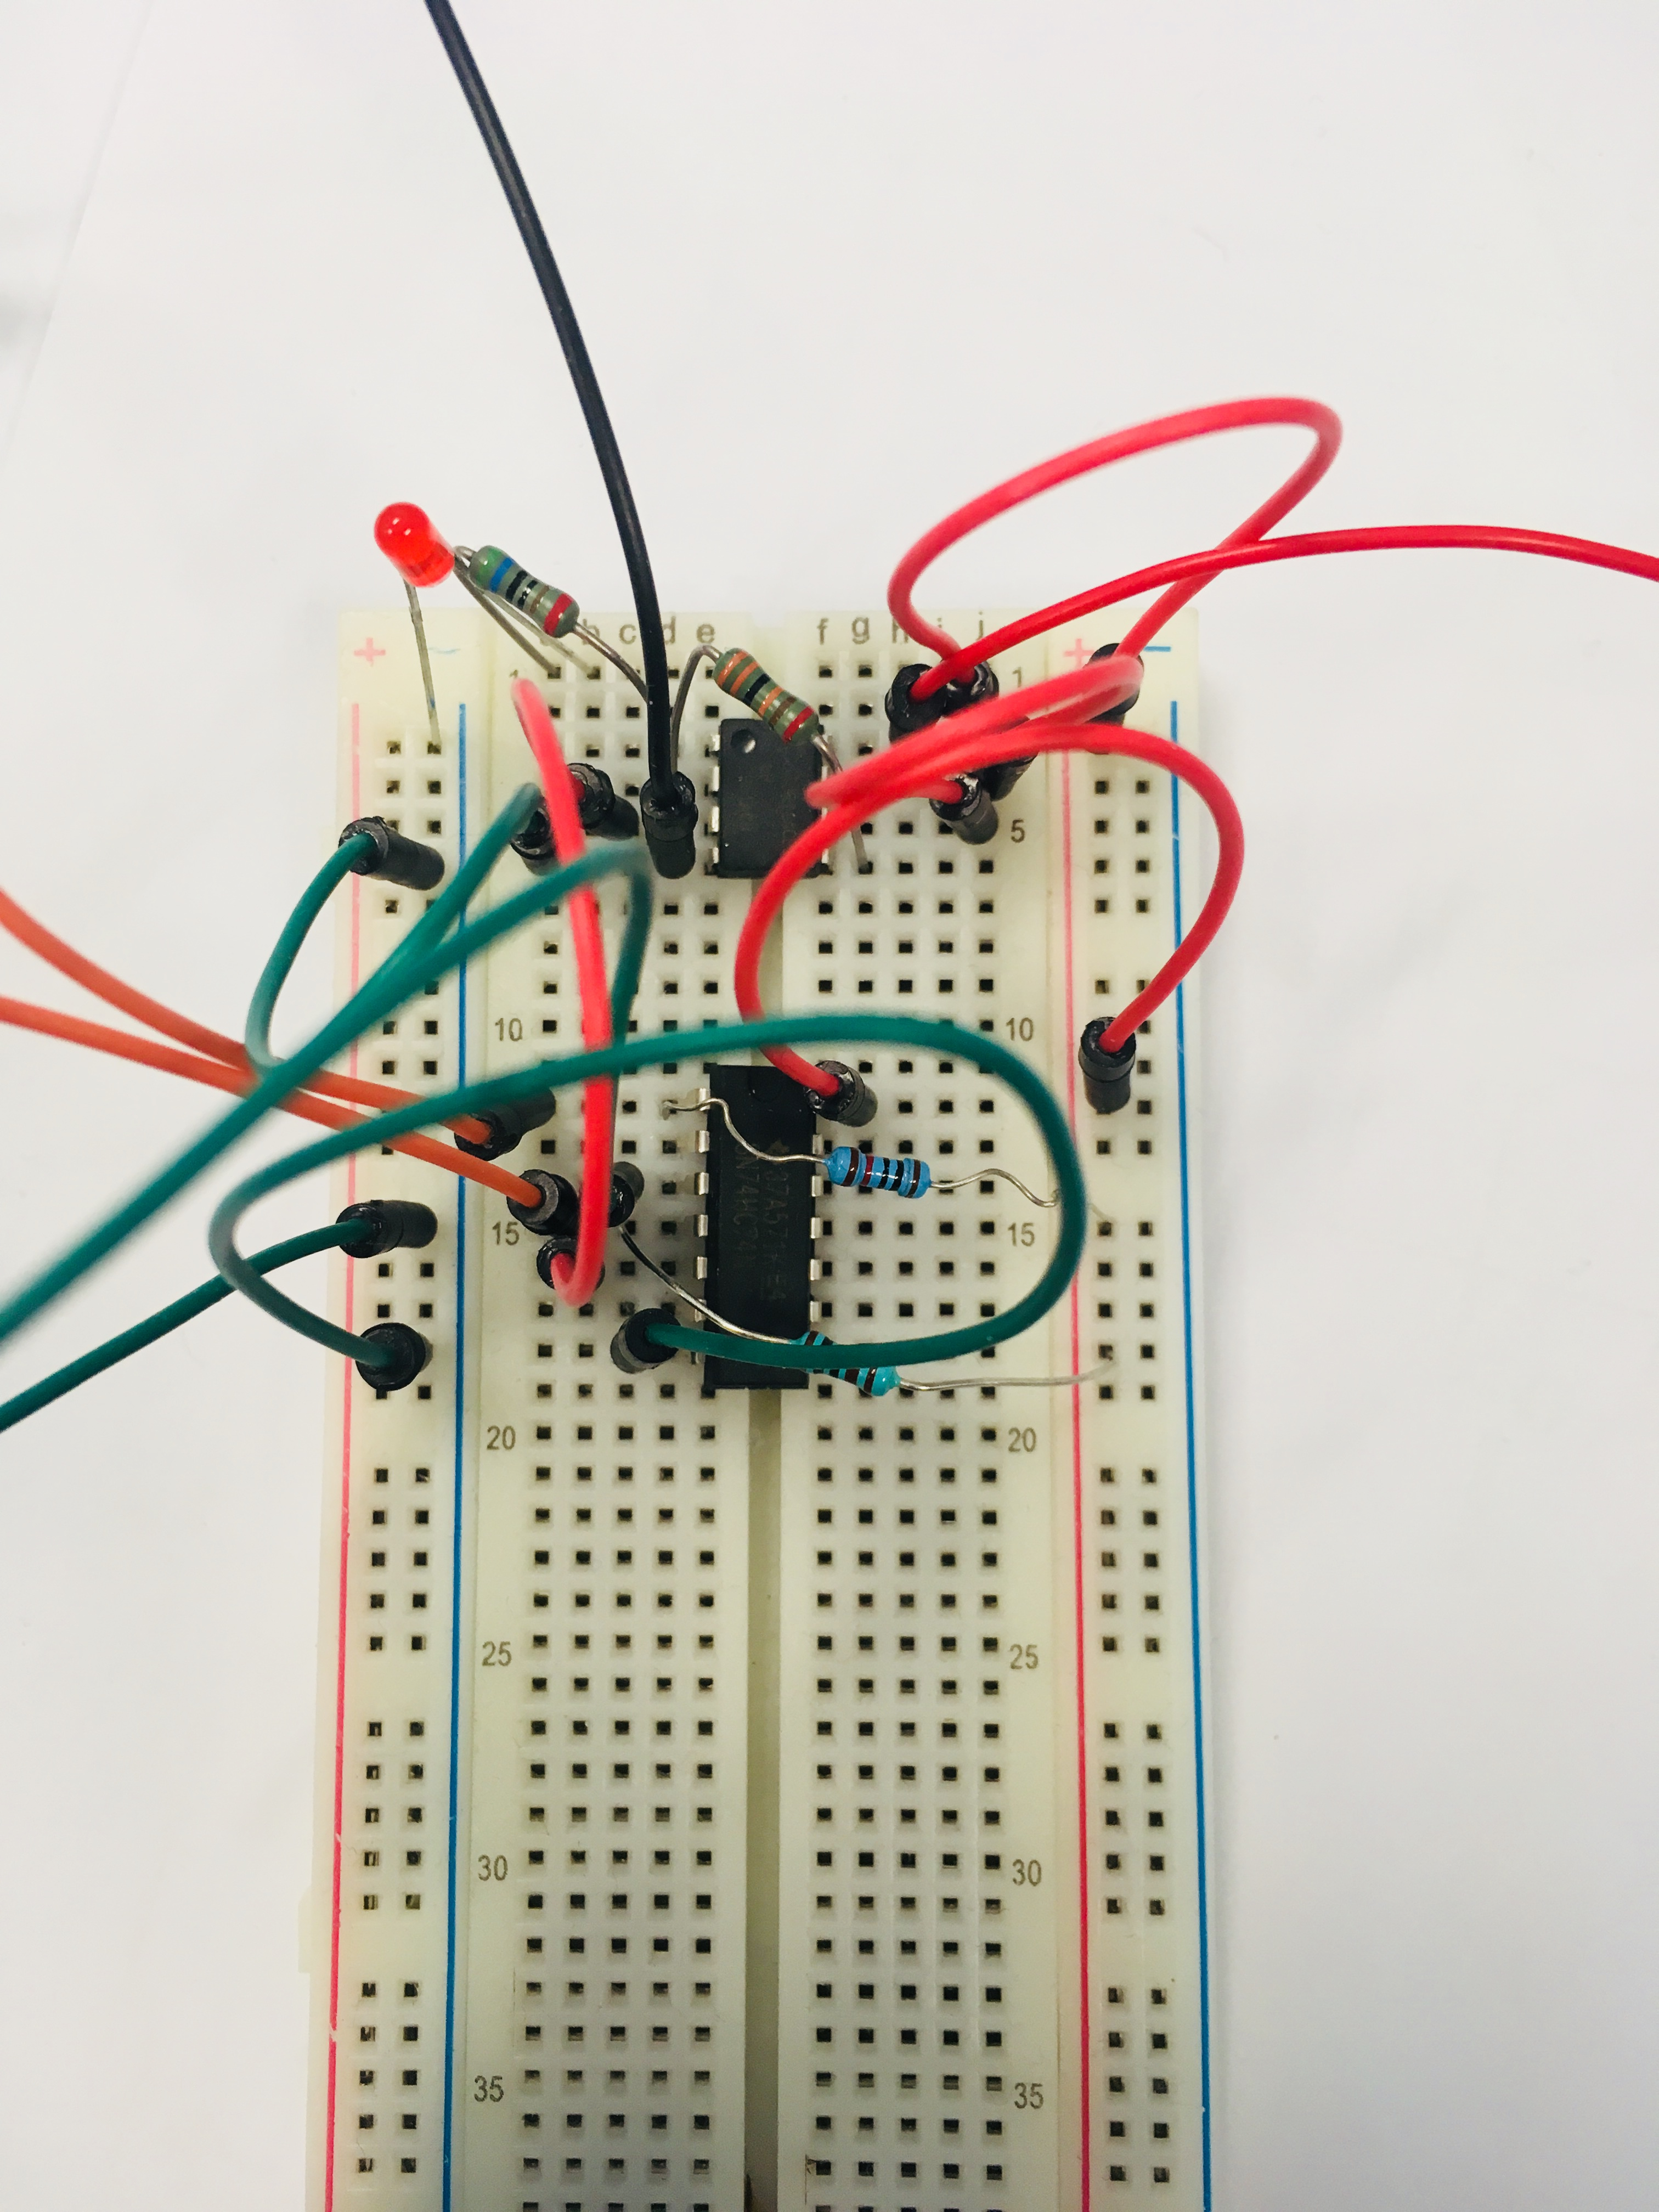
\includegraphics[width=0.5\linewidth]{powercircuit.jpg}\centering
	\caption{Image of test power circuit}
	\label{fig:power_circuit}
\end{figure}


%----------------------------------------------------------------------------------------


